\documentclass[10pt,aspectratio=169]{beamer}

\usetheme{metropolis}
\metroset{sectionpage=none}

\usepackage{amsmath,amssymb,amsfonts}
\usepackage{bm}
\usepackage{booktabs}
\usepackage{tikz}
\usepackage{xcolor}
\usetikzlibrary{arrows.meta, positioning, shapes.geometric, fit, backgrounds}

% Useful macros
\newcommand{\T}{\mathcal{T}}
\newcommand{\Hh}{\mathcal{H}}
\newcommand{\E}{\mathbb{E}}
\newcommand{\R}{\mathbb{R}}
\newcommand{\N}{\mathcal{N}}
\newcommand{\indep}{\perp\!\!\!\perp}

\title{Horseshoe Forests for High-Dimensional\\ Causal Survival Analysis}
\subtitle{ISBA World Meeting}
\date{}
\author{Tijn Jacobs \\
\small joint work with Wessel N.\ van Wieringen and St\'ephanie L.\ van der Pas}
\institute{Vrije Universiteit Amsterdam}


\definecolor{myaccent}{HTML}{0077B3}
\setbeamercolor{alerted text}{fg=myaccent}        % \alert{}, alertblock borders
\setbeamercolor{progress bar}{fg=myaccent}        % progressbar if enabled
\setbeamercolor{frametitle}{bg=myaccent, fg=white} % solid-colour frame title bar
\setbeamercolor{normal text}{fg=black!90, bg=white}

\usepackage{graphicx}
\usepackage{qrcode}
\titlegraphic{%
  \vspace{6.5cm}%  push it down toward the bottom
  \hfill
\includegraphics[height=1cm]{VU-logo-CMYK.pdf}%
}
\begin{document}

\maketitle

%---------------------------------------------------------
\begin{frame}{This talk in one slide}
\textbf{Goal.} Estimate heterogeneous causal effects of a binary treatment on a censored survival outcome when the number of covariates is large ($p \gg n$).
\bigskip

\textbf{Idea.} Take the BART prior and \emph{move the regularisation from the tree structure to the leaf parameters} via a horseshoe prior on the step heights.
\bigskip

\textbf{Cost.} Conjugacy is lost $\Rightarrow$ reversible-jump-within-Gibbs sampler with a tailored proposal.
\bigskip

\textbf{Pay-off.}
\begin{itemize}
  \item Stable RMSE and near-nominal coverage as $p$ grows.
  \item Robust to regularisation-induced confounding.
  \item Application: adjuvant radiotherapy in pancreatic cancer (TCGA-PAAD).
\end{itemize}
\end{frame}

%---------------------------------------------------------
\section{Problem setup}

\begin{frame}{The setting}
\begin{columns}[T,onlytextwidth]
\begin{column}{0.70\textwidth}
\textbf{Observational survival data} $(Y_i, \delta_i, A_i, X_i)$, $i=1,\ldots,n$:
\begin{itemize}
  \item $Y_i = \min(T_i, C_i)$, $\delta_i = \mathbf{1}\{T_i \le C_i\}$ \quad (right-censored)
  \item $A_i \in \{0,1\}$ \quad (binary, non-randomised)
  \item $X_i \in \R^p$ \quad with $p \gg n$
\end{itemize}
\end{column}
\begin{column}{0.30\textwidth}
\centering
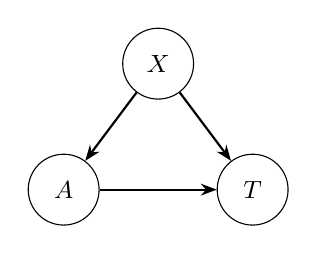
\begin{tikzpicture}[
  node distance=1.2cm,
  every node/.style={circle, draw, minimum size=0.9cm, font=\small},
  arr/.style={-{Stealth[length=2mm]}, thick}
]
\node (X) at (0,1.2) {$X$};
\node (A) at (-1.2,-0.4) {$A$};
\node (T) at (1.2,-0.4) {$T$};
\draw[arr] (X) -- (A);
\draw[arr] (X) -- (T);
\draw[arr] (A) -- (T);
\end{tikzpicture}
\end{column}
\end{columns}

\bigskip

\textbf{Question.} What is the causal effect of $A$ on $T$ given $X$, allowing for heterogeneity across patients?
\bigskip

\textbf{Estimand.} The conditional average treatment effect on the log-survival scale,
\[
\tau(x) \;:=\; \E\left[\log T(1) - \log T(0)\,\big|\, X = x\right].
\]
\end{frame}

%---------------------------------------------------------
\begin{frame}{Identification assumptions}
Potential-outcomes framework $\bigl(T(a), C(a)\bigr)$. Identification proceeds in two steps.

\medskip

\textbf{1. Causal assumptions} --- link potential outcomes to observables:
\begin{itemize}
  \item \textit{SUTVA}: no interference, well-defined potential outcomes.
  \item \textit{Unconfoundedness}: $T(a) \indep A \mid X$.
  \item \textit{Positivity}: $0 < e(x) := P(A{=}1 \mid X{=}x) < 1$.
\end{itemize}


\vspace{0.6cm}
\textbf{2. Censoring assumption} --- makes the distribution of $T \mid X, A$ identifiable from the censored data $(Y,\delta)$:
\begin{itemize}
  \item \textit{Independent censoring}: $C(a) \indep T(a) \mid X, A$.
\end{itemize}


\end{frame}

%---------------------------------------------------------
\begin{frame}{An accelerated failure time decomposition}
We model the log-event times:
\[
\log T(a) \;=\; f\bigl(x, \hat e(x)\bigr) \;+\; a \cdot \tau(x) \;+\; \varepsilon, \qquad \varepsilon \;\sim\; \N(0, \sigma^2).
\]

\begin{itemize}
  \item $f$: prognostic function.
  \item $\hat e(x)$: estimated propensity score.
  \item $\tau(x)$: heterogeneous treatment effect.
\end{itemize}
\bigskip

\textbf{Why AFT here?} AFT effects are collapsible: the marginal effect is the average of conditional effects.

\bigskip
\textbf{Plan.} Place a flexible Bayesian tree-ensemble prior on both $f$ and $\tau$, separately.
\end{frame}

%---------------------------------------------------------
\section{From BART to Horseshoe Forests}

\begin{frame}{BART in one slide}
\begin{center}
\begin{minipage}[c]{0.38\linewidth}
  \centering
  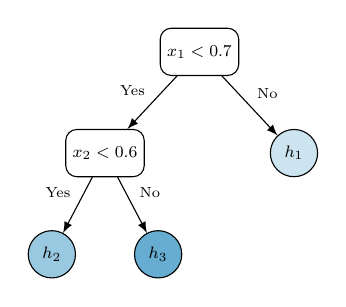
\begin{tikzpicture}[
        scale=0.75, transform shape,
        box/.style={rectangle, draw, rounded corners, align=center, minimum height=8mm, minimum width=13mm, font=\footnotesize},
        leaf/.style={circle, draw, align=center, minimum size=8mm, font=\footnotesize},
        line/.style={-latex}
    ]
    \node [box] (root) {$x_1 < 0.7$};
    \node [box, below=0.9cm of root, xshift=-1.6cm] (left) {$x_2 < 0.6$};
    \node [leaf, fill=myaccent!20, below=0.9cm of root, xshift=1.6cm] (h1) {$h_1$};
    \node [leaf, fill=myaccent!40, below=0.9cm of left, xshift=-0.9cm] (h2) {$h_2$};
    \node [leaf, fill=myaccent!60, below=0.9cm of left, xshift=0.9cm] (h3) {$h_3$};
    \draw[line] (root) -- (left) node[midway, above left, font=\scriptsize] {Yes};
    \draw[line] (root) -- (h1) node[midway, above right, font=\scriptsize] {No};
    \draw[line] (left) -- (h2) node[midway, above left, font=\scriptsize] {Yes};
    \draw[line] (left) -- (h3) node[midway, above right, font=\scriptsize] {No};
  \end{tikzpicture}
\end{minipage}\hfill
\begin{minipage}[c]{0.08\linewidth}
  \centering
  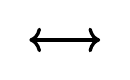
\begin{tikzpicture}
    \draw[<->, very thick] (0,0) -- (0.9,0);
  \end{tikzpicture}
\end{minipage}\hfill
\begin{minipage}[c]{0.38\linewidth}
  \centering
  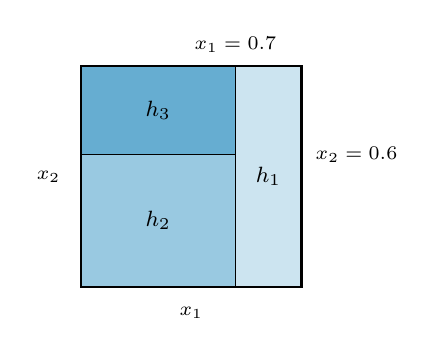
\begin{tikzpicture}[scale=2.8]
    \fill[myaccent!20] (0.7, 0) rectangle (1, 1);
    \fill[myaccent!40] (0, 0)   rectangle (0.7, 0.6);
    \fill[myaccent!60] (0, 0.6) rectangle (0.7, 1);
    \draw[thick] (0, 0) rectangle (1, 1);
    \draw[thin] (0.7, 0) -- (0.7, 1);
    \draw[thin] (0, 0.6) -- (0.7, 0.6);
    \node[below, font=\scriptsize] at (0.5, -0.05) {$x_1$};
    \node[left, font=\scriptsize] at (-0.05, 0.5) {$x_2$};
    \node[right, font=\scriptsize] at (1.02, 0.6) {$x_2 = 0.6$};
    \node[above, font=\scriptsize] at (0.7, 1.02) {$x_1 = 0.7$};
    \node[font=\footnotesize] at (0.85, 0.5) {$h_1$};
    \node[font=\footnotesize] at (0.35, 0.3) {$h_2$};
    \node[font=\footnotesize] at (0.35, 0.8) {$h_3$};
  \end{tikzpicture}
\end{minipage}
\end{center}


\vspace{-0.2em}

\textbf{Model.} $g(x) = \sum_{j=1}^{m} g(x;\, \T_j, \Hh_j)$ --- a sum of many shallow trees, each piecewise constant on a partition of the covariate space.

\vspace{0.3cm}

\textbf{Prior.}
\begin{itemize}
  \item Tree shape $\T_j$: depth-penalised Galton--Watson.
  \item Step heights $\Hh_j$: i.i.d.\ Gaussian, variance $\propto 1/m$.
\end{itemize}

\end{frame}

%---------------------------------------------------------
\begin{frame}{Where does regularisation come from in BART?}
Two places to regularise a tree ensemble:

\bigskip

\begin{enumerate}
  \item \textbf{Via the tree structure} $\T_j$ --- depth penalty, splitting rules, covariate selection (DART, Soft-BART, \ldots).
  \medskip
  \item \textbf{Via the step heights} $\Hh_j$ --- shrink the \emph{magnitudes} of step heights.
\end{enumerate}

\bigskip

Existing work focuses on (1), but controlling tree structure alone is not enough in high dimensions, or induces bias by dropping relevant confounders.
\bigskip

\textbf{Novel contribution.} Regularise through (2): a global--local shrinkage prior on the step heights.
\end{frame}

%---------------------------------------------------------
\begin{frame}{Horseshoe prior on the step heights}
\begin{columns}[T,onlytextwidth]
\begin{column}{0.55\textwidth}
For a tree with step heights $\ell = 1,\ldots, L$:
\[
h_\ell \mid \lambda_\ell^2, \gamma^2 \;\sim\; \N\bigl(0,\, \lambda_\ell^2\, \gamma^2\bigr),
\]
\[
\lambda_\ell \;\sim\; \mathcal{C}^+(0, 1), \qquad \gamma \;\sim\; \mathcal{C}^+(0, 1).
\]

\vspace{0.8cm}

\textbf{Global--local shrinkage:}
\begin{itemize}
  \item $\gamma$ pulls \emph{everything} to zero.
  \item $\lambda_\ell$ lets individual step heights \emph{escape} locally.
\end{itemize}

\smallskip
\textit{$\Rightarrow$ regularise globally, pick up signals locally.}
\end{column}
\begin{column}{0.45\textwidth}
\centering
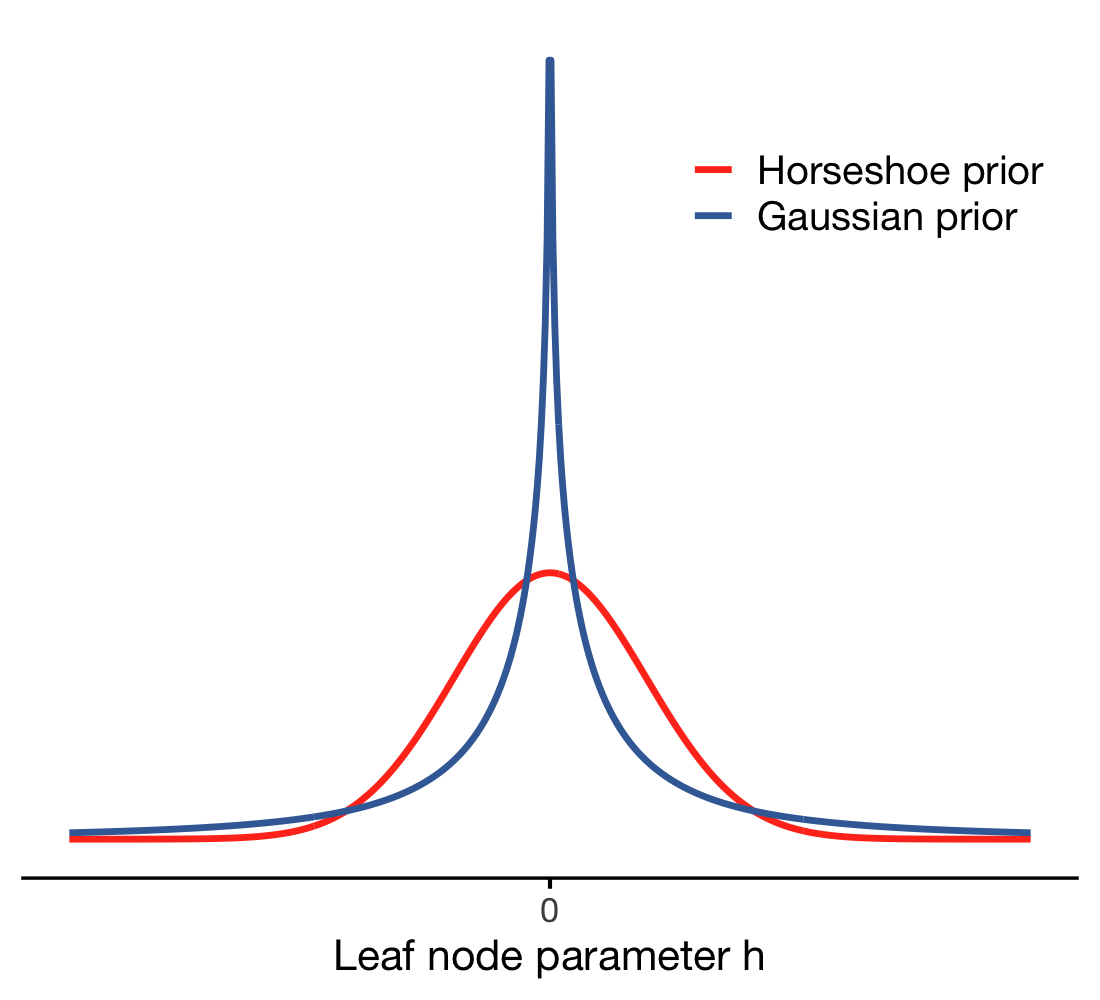
\includegraphics[width=\linewidth]{Horseshoe_plot_ICSDS.png}
\end{column}
\end{columns}
\end{frame}

%---------------------------------------------------------
\section{Posterior inference}

\begin{frame}{Inference: reversible-jump on trees}
\begin{columns}[c,onlytextwidth]
\begin{column}{0.38\textwidth}
The horseshoe prior on step heights is not Gaussian-conjugate $\Rightarrow$ step heights cannot be marginalised out.

\vspace{0.5cm}

GROW and PRUNE change the dimension of $\Hh_j$. We use a \textbf{reversible-jump} step with a tailored proposal for $(\T_j, \Hh_j)$.

\vspace{0.5cm}

This sits inside a Gibbs sampler that updates the forests $f$ and $\tau$, the error variance $\sigma^2$, and the augmented censored event times.
\end{column}
\begin{column}{0.58\textwidth}
\centering
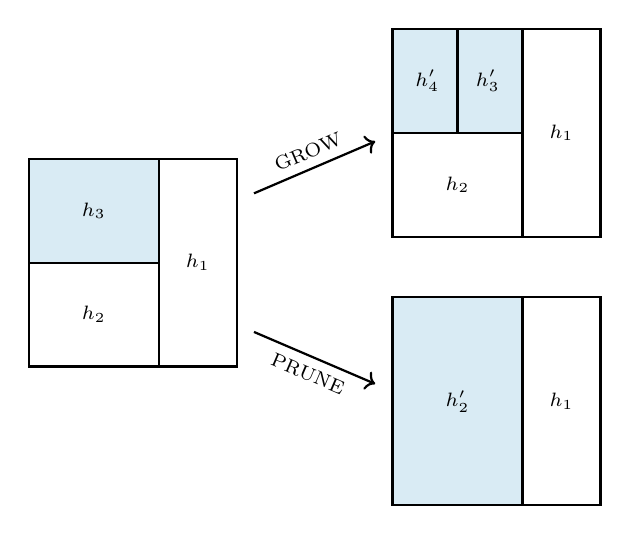
\begin{tikzpicture}[
  scale=1.1,
  every node/.style={font=\scriptsize}
]
% Parent partition — highlight the cell about to be split
\fill[myaccent!15] (0,1.2) rectangle (1.5,2.4);
\draw[thick] (0,0) rectangle (2.4,2.4);
\draw[thick] (1.5,0) -- (1.5,2.4);
\draw[thick] (0,1.2) -- (1.5,1.2);
\node at (0.75,1.8) {$h_3$};
\node at (0.75,0.6) {$h_2$};
\node at (1.95,1.2) {$h_1$};

\draw[->, thick] (2.6,2.0) -- (4.0,2.6) node[midway, above, sloped] {GROW};
\draw[->, thick] (2.6,0.4) -- (4.0,-0.2) node[midway, below, sloped] {PRUNE};

% GROW result — highlight the newly split children
\begin{scope}[shift={(4.2,1.5)}]
\fill[myaccent!15] (0,1.2) rectangle (1.5,2.4);
\draw[thick] (0,0) rectangle (2.4,2.4);
\draw[thick] (1.5,0) -- (1.5,2.4);
\draw[thick] (0,1.2) -- (1.5,1.2);
\draw[thick] (0.75,1.2) -- (0.75,2.4);
\node at (0.4,1.8) {$h'_4$};
\node at (1.1,1.8) {$h'_3$};
\node at (0.75,0.6) {$h_2$};
\node at (1.95,1.2) {$h_1$};
\end{scope}

% PRUNE result — highlight the merged cell
\begin{scope}[shift={(4.2,-1.6)}]
\fill[myaccent!15] (0,0) rectangle (1.5,2.4);
\draw[thick] (0,0) rectangle (2.4,2.4);
\draw[thick] (1.5,0) -- (1.5,2.4);
\node at (0.75,1.2) {$h'_2$};
\node at (1.95,1.2) {$h_1$};
\end{scope}
\end{tikzpicture}
\end{column}
\end{columns}
\end{frame}

%---------------------------------------------------------
\section{Simulations}

\begin{frame}{Simulation 1: CATE estimation as $p$ grows}
Non-linear treatment effect with sparse main (5\%) + interaction (1\%)  structure; $n = 200$, $p \in [50, 5000]$, censoring $\approx 35\%$.

\vspace{-0.3em}
\begin{center}
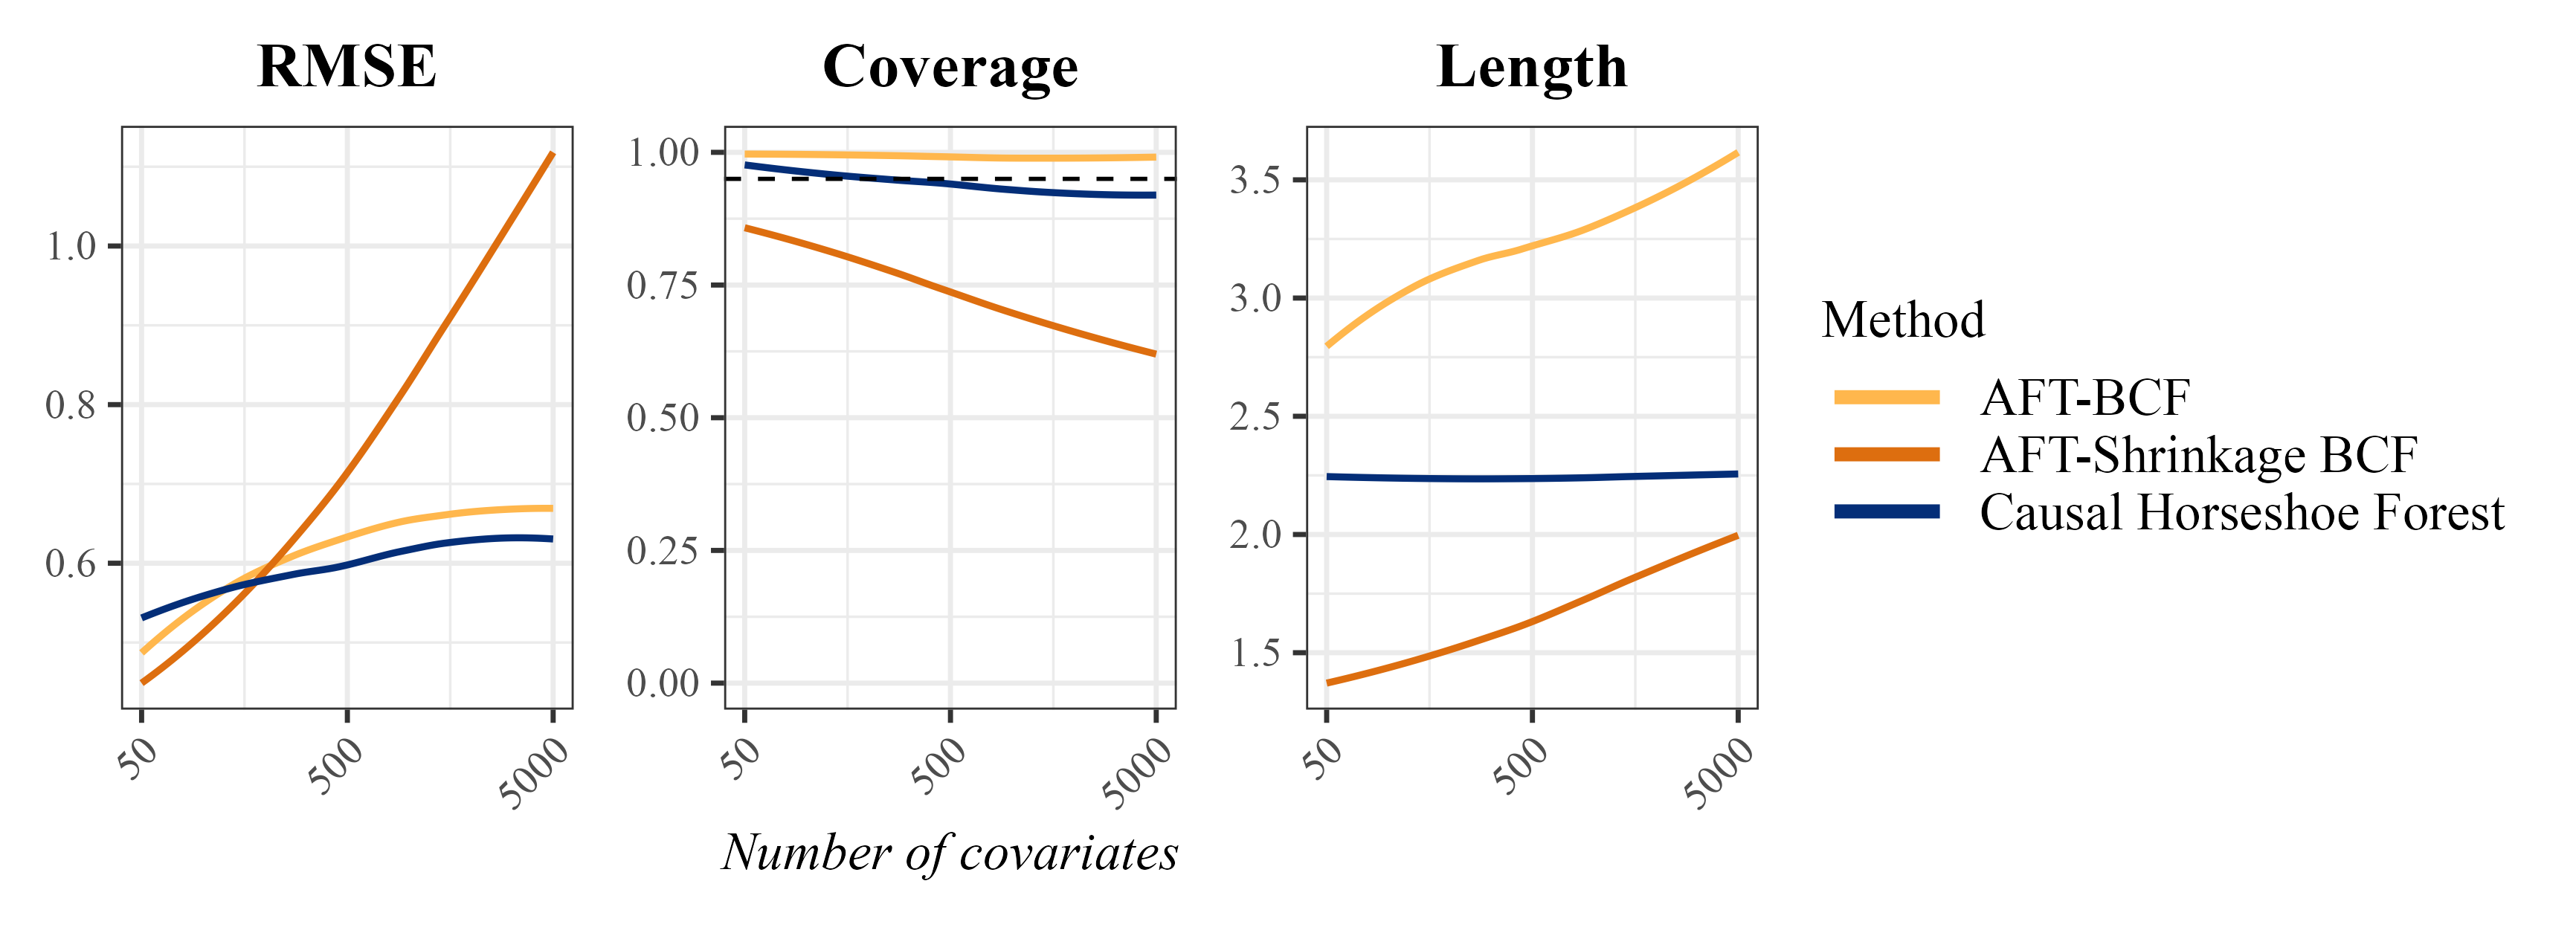
\includegraphics[width=0.95\linewidth]{revision_main_deeper.png}
\end{center}
\end{frame}

%---------------------------------------------------------
\begin{frame}{Simulation 2: regularisation-induced confounding}
$n = 100$, $p = 500$, censoring $\approx 35\%$. Two groups of confounders:
\begin{itemize}
  \item $|S| = 5$ \textbf{strong} confounders --- contribute substantially to both treatment and outcome.
  \item $|W| \in \{1, \ldots, 20\}$ \textbf{weak} confounders --- predict treatment, but contribute only weakly to the outcome.
\end{itemize}



\vspace{0.2cm}
\begin{center}
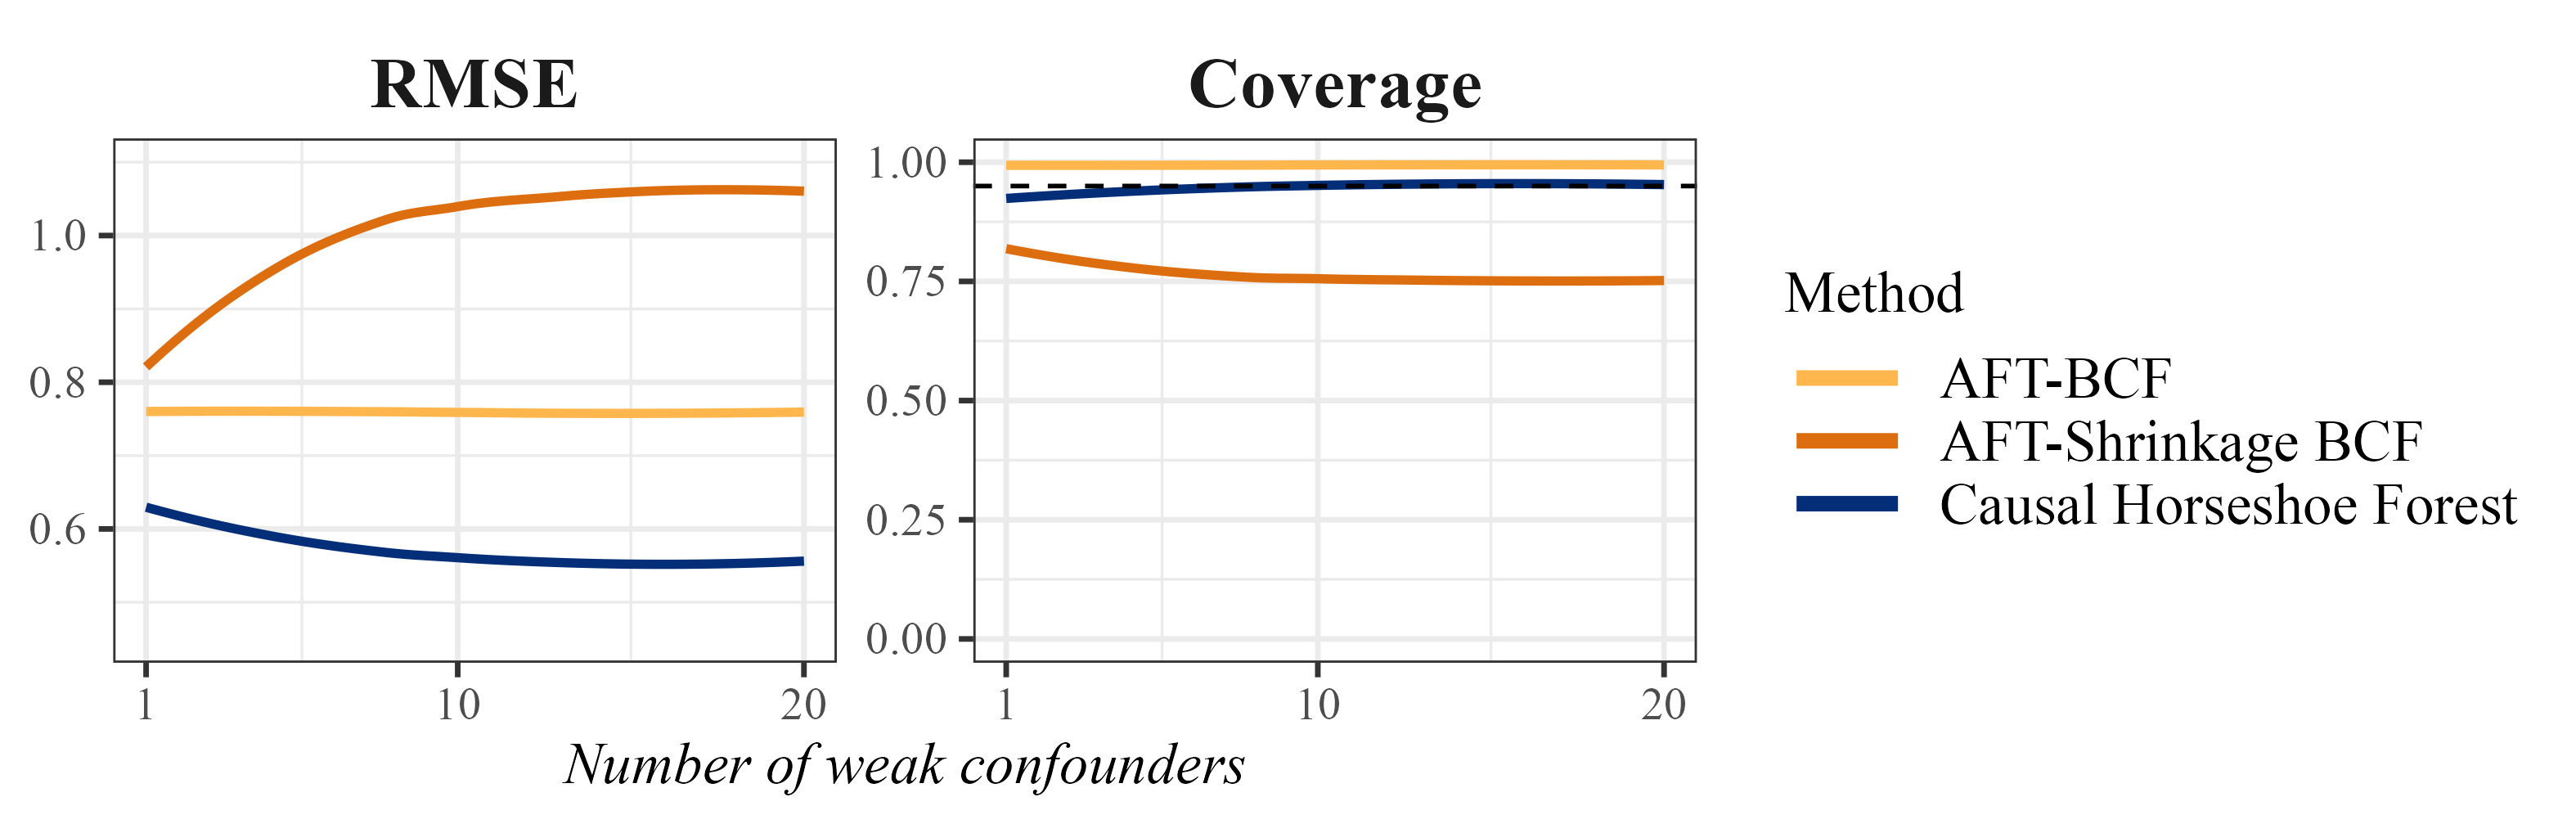
\includegraphics[width=0.95\linewidth]{revision_ric.png}
\end{center}
\end{frame}

%---------------------------------------------------------
\section{Application: pancreatic cancer}

\begin{frame}{Adjuvant radiotherapy in PDAC}
\begin{columns}[T,onlytextwidth]
\begin{column}{0.40\textwidth}
\textbf{Data.} TCGA-PAAD, $n = 130$ resected PDAC patients.
\begin{itemize}
  \item \textit{Outcome}: overall survival; censoring $\approx 47\%$, median follow-up 23.3 mo.
  \item \textit{Treatment}: adjuvant radiotherapy.
  \item \textit{Covariates}: 11 clinical $+$ driver genes $+$ top 3{,}000 genes by MAD ($p \approx 3{,}029$).
\end{itemize}
\end{column}
\begin{column}{0.60\textwidth}
\centering
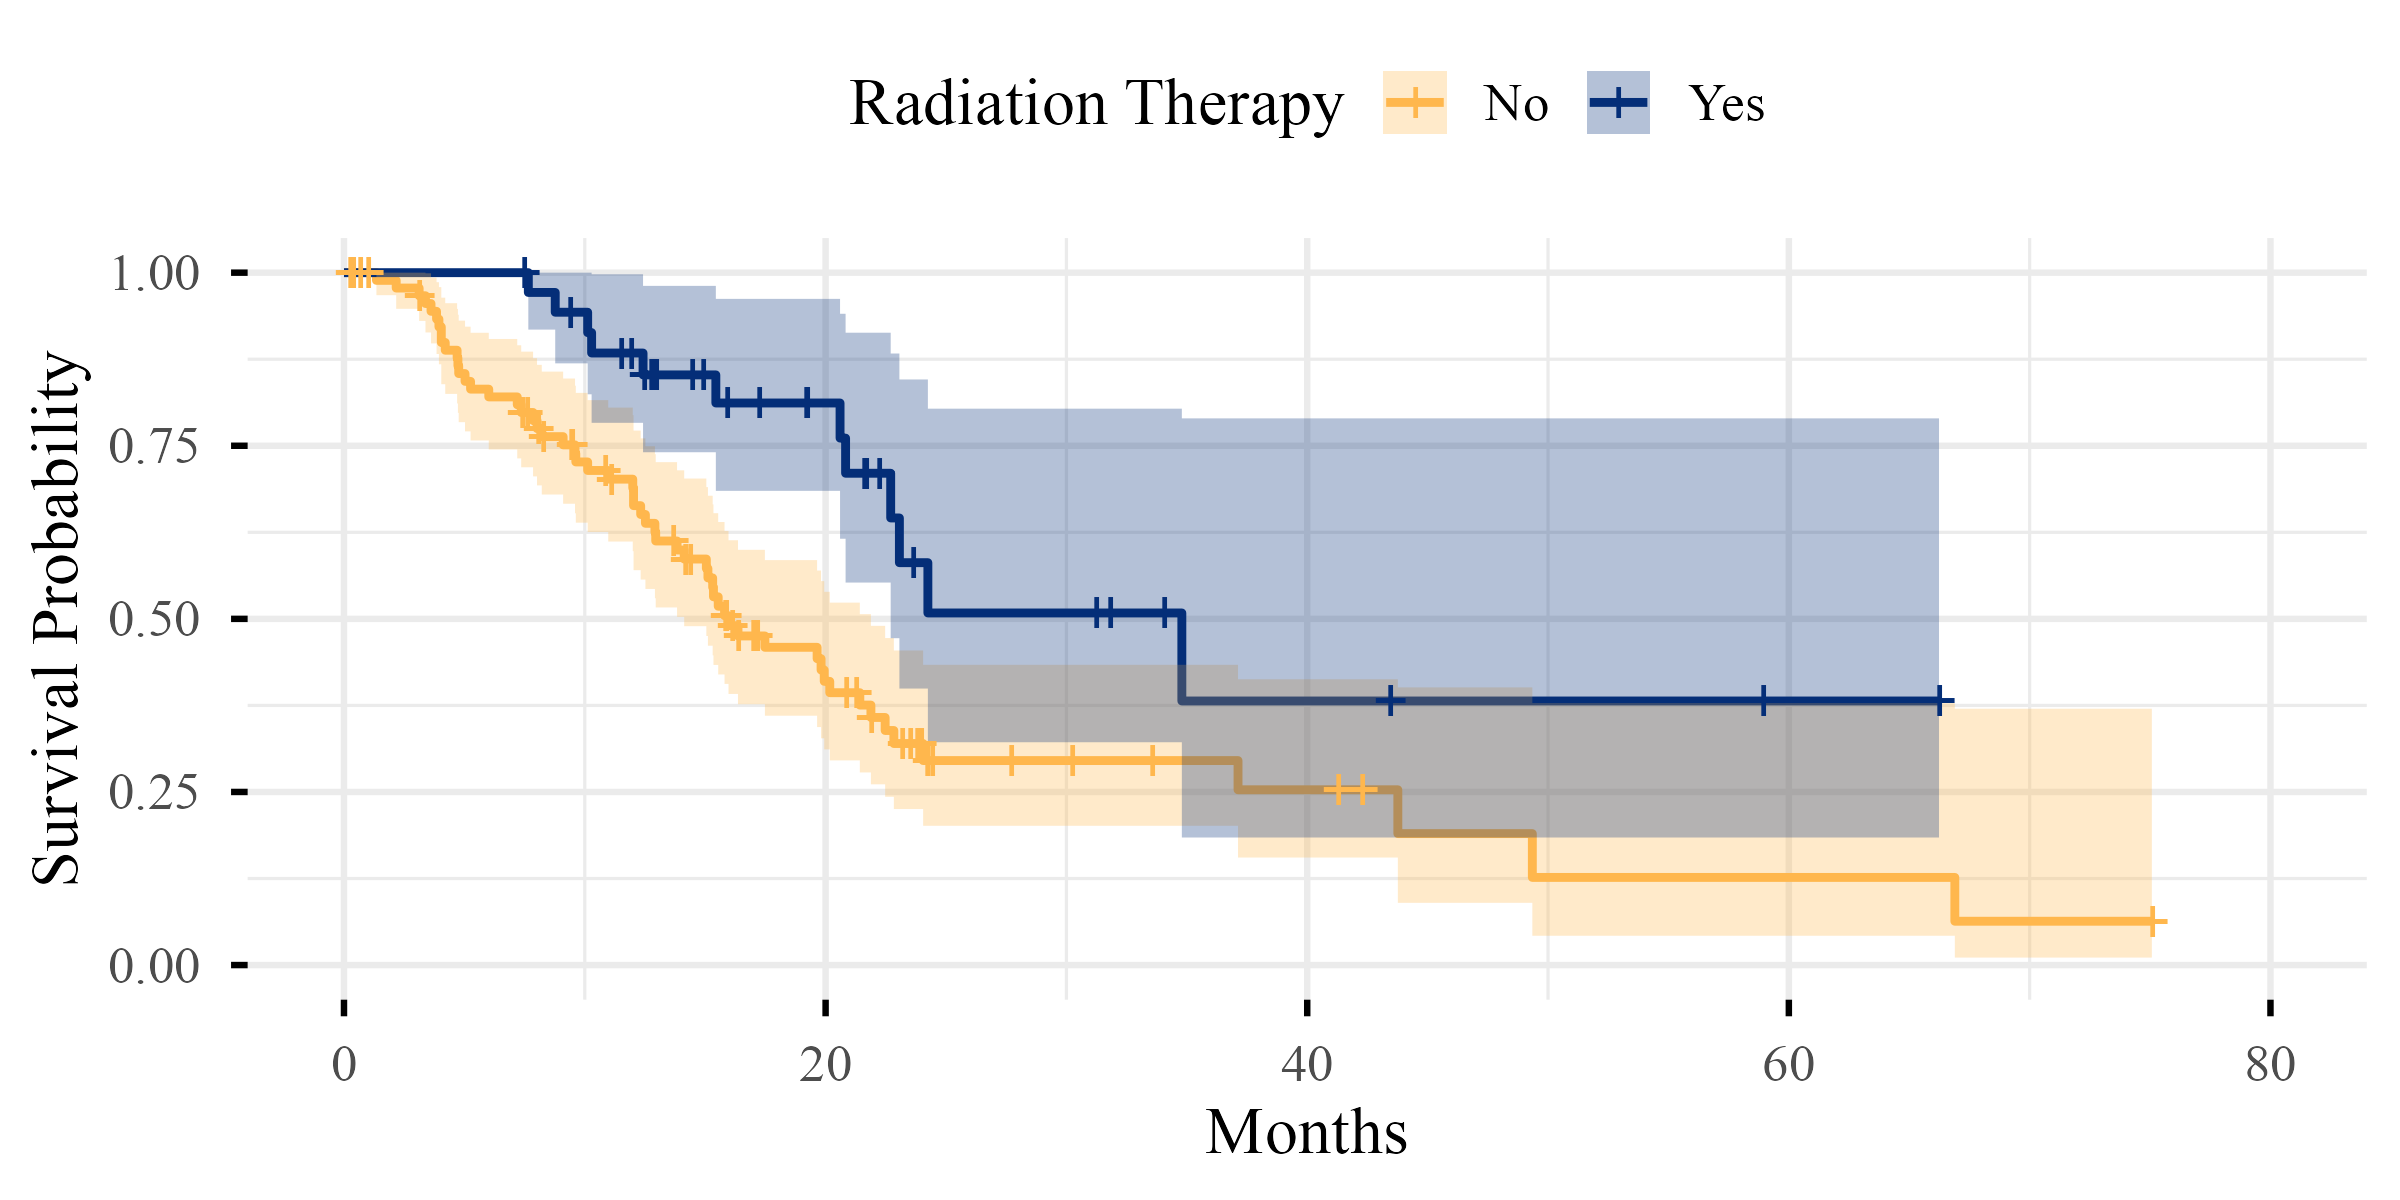
\includegraphics[width=\linewidth]{PDAC_KaplanMeier.png}
\end{column}
\end{columns}


\bigskip

\textbf{Question.} Does adjuvant radiotherapy improve survival, and is the effect heterogeneous?

\end{frame}

%---------------------------------------------------------
\begin{frame}{Adjuvant radiotherapy in PDAC}
\begin{columns}[c,onlytextwidth]
\begin{column}{0.5\textwidth}
\centering
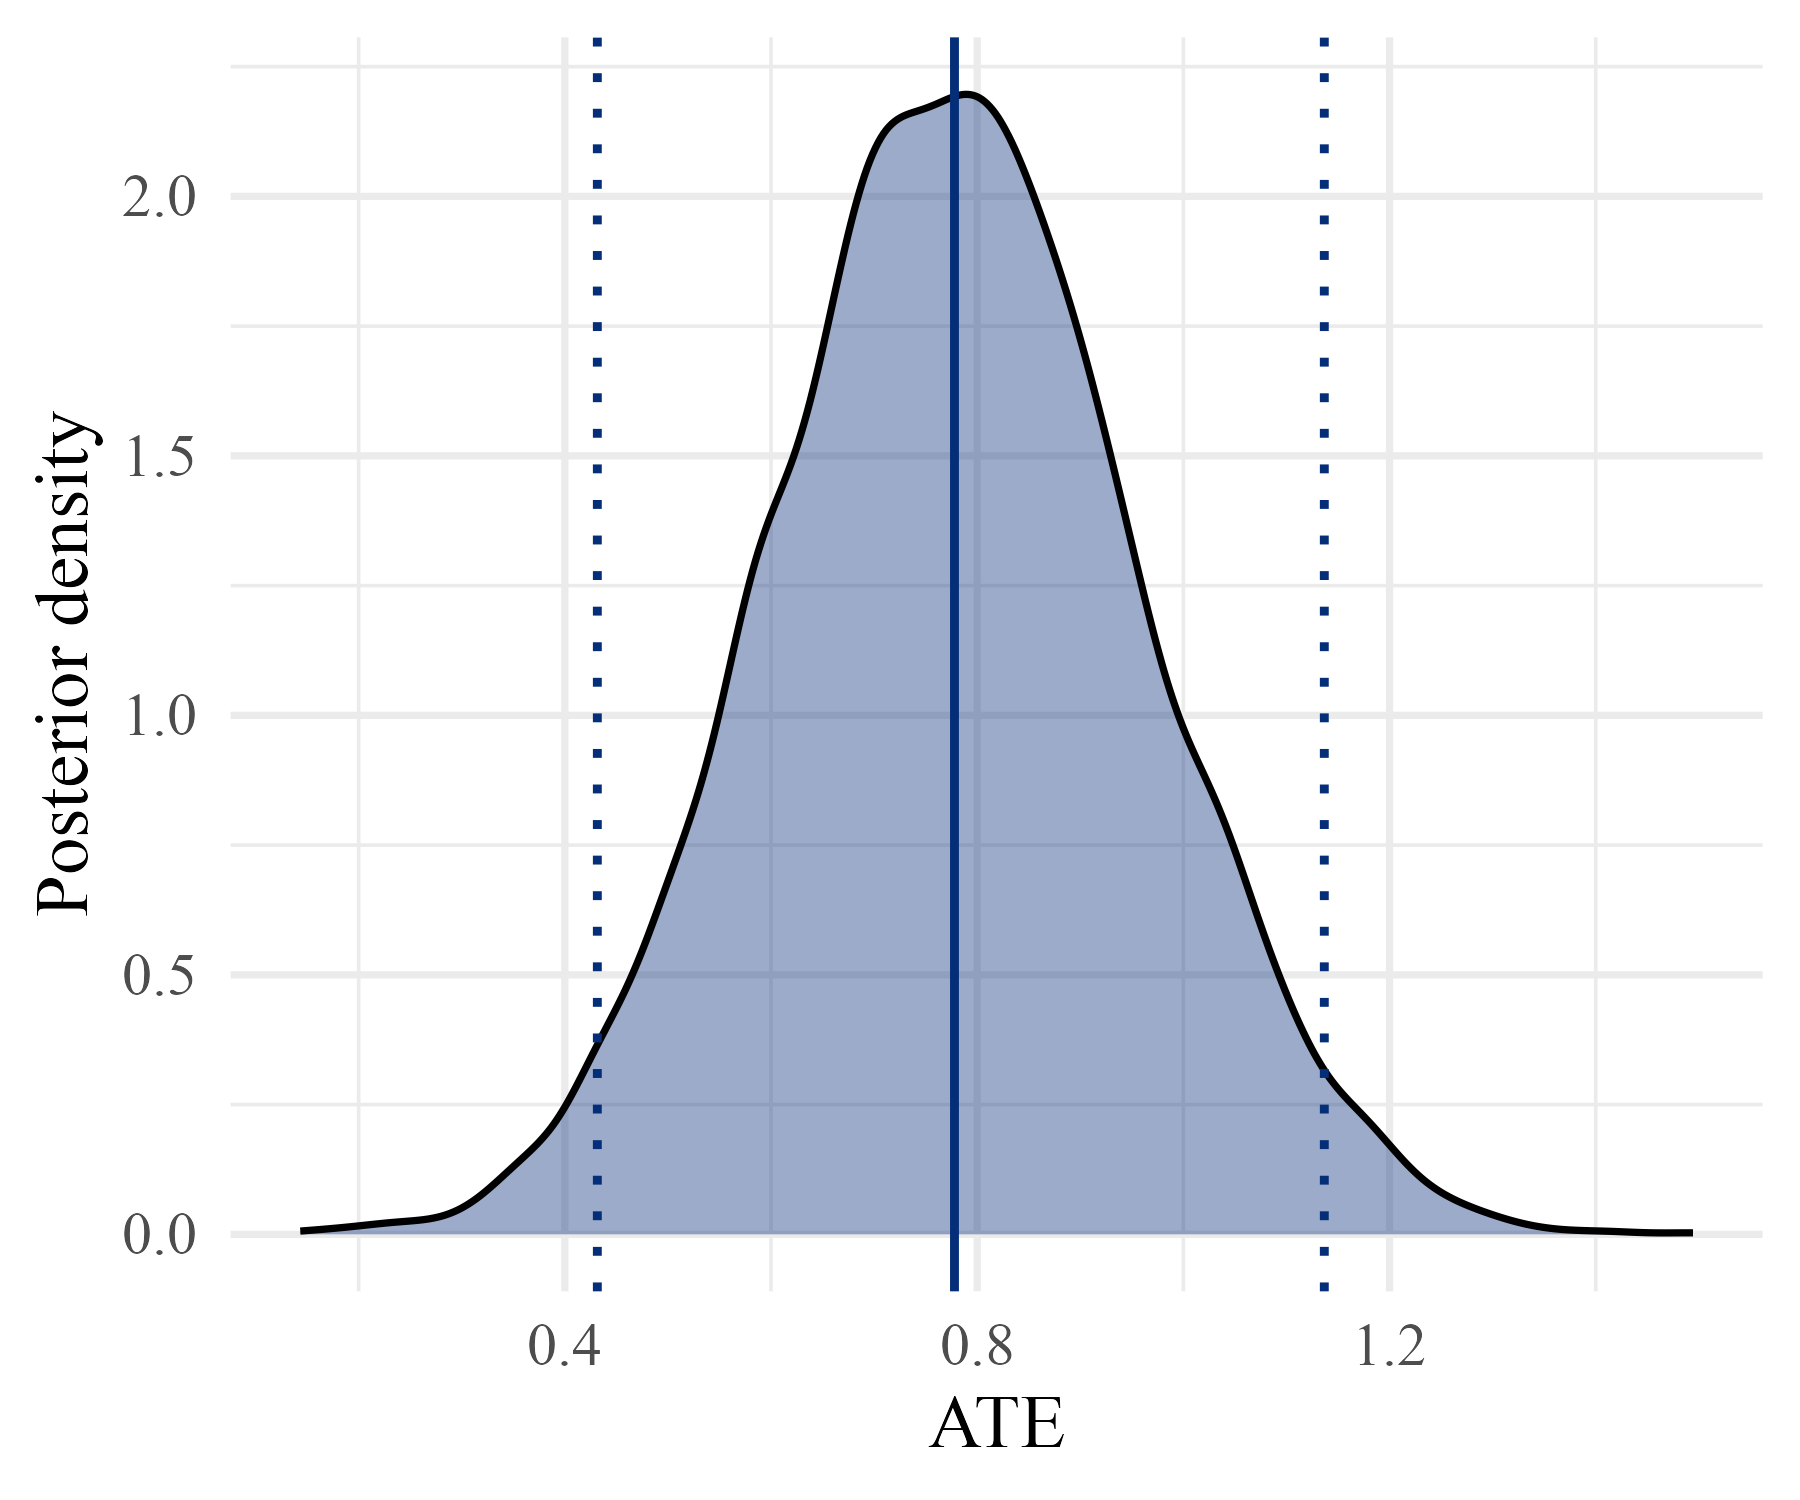
\includegraphics[width=\linewidth]{Plot_posteriorATE.png}

\smallskip
{\footnotesize $\widehat{\text{ATE}} \approx 0.75$, \, 95\% CrI $(0.40,\, 1.11)$.}
\end{column}
\begin{column}{0.5\textwidth}
\centering
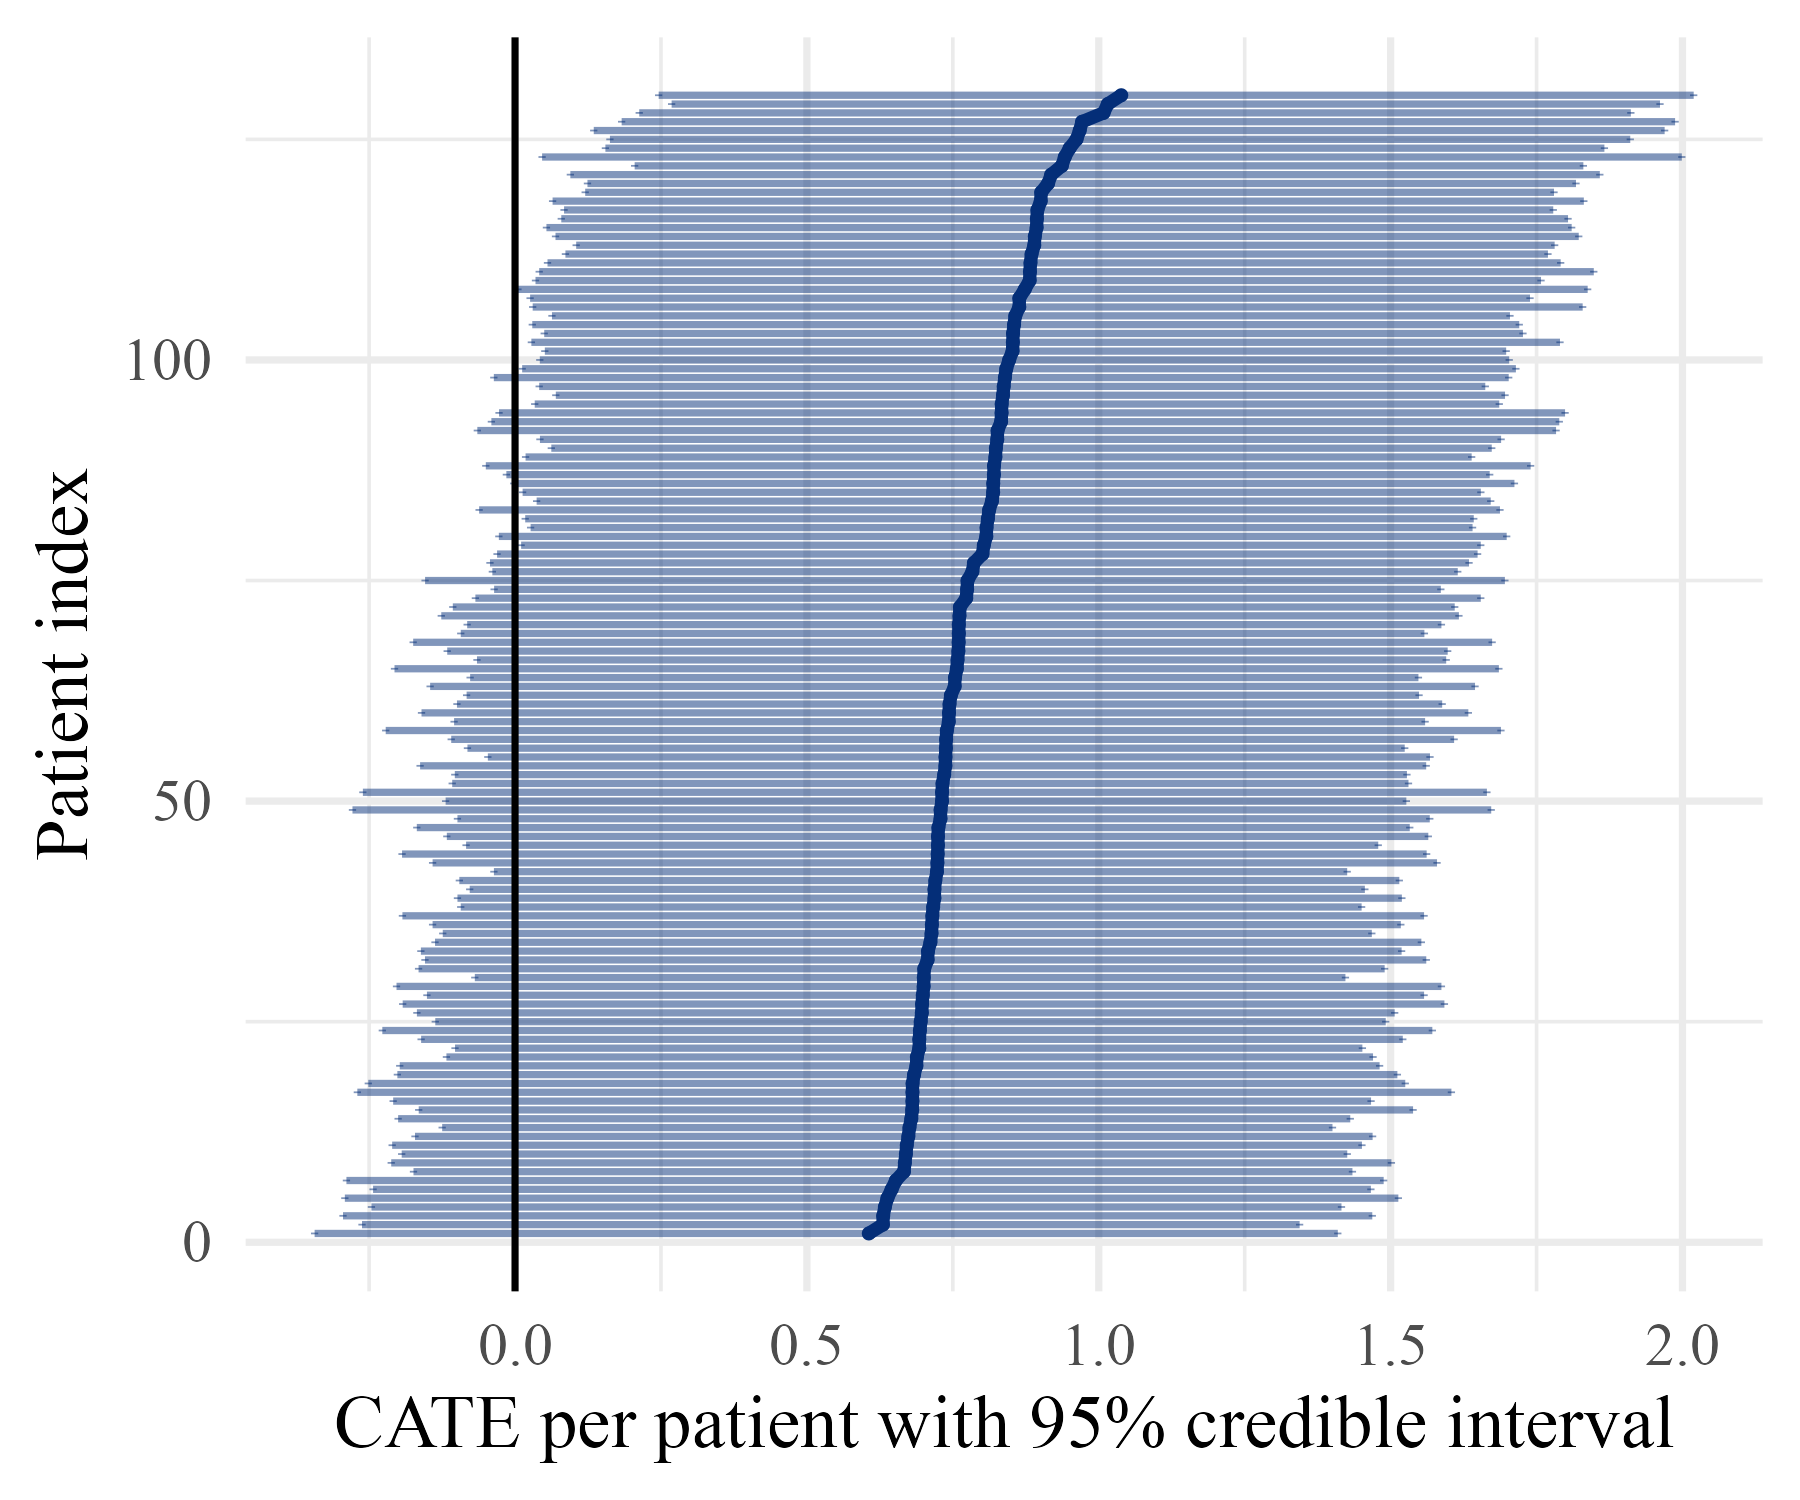
\includegraphics[width=\linewidth]{plot_CATEpatient.png}

\smallskip
{\footnotesize $\approx 96.9\%$ of patients have $P(\tau(X_i) > 0 \mid \text{data}) > 0.95$.}
\end{column}
\end{columns}
\end{frame}

%---------------------------------------------------------
\section{Wrap-up}

\begin{frame}{Take-aways}
\begin{itemize}
\item \textbf{Where you regularise matters.} Shifting the regularisation from the tree structure onto the \emph{step heights} of a tree ensemble gives a flexible, adaptive prior for high-dimensional CATE estimation.  \vspace{0.3cm}
  \item \textbf{The price is a reversible-jump sampler.} A tailored tree proposal keeps the chain mixing well.
  \vspace{0.3cm}
  \item \textbf{Strong empirical performance.} Stable RMSE and near-nominal coverage as $p$ grows; robust to regularisation-induced confounding where competing methods break down.
\end{itemize}
\end{frame}

%---------------------------------------------------------
\begin{frame}{Thank you}
\begin{columns}[c,onlytextwidth]
\begin{column}{0.62\textwidth}
\begin{itemize}
  \item Preprint on arXiv: \texttt{2507.22004}.
  \item R package \textbf{ShrinkageTrees} on CRAN (and GitHub).
  \item Questions? \texttt{t.jacobs@vu.nl}.
\end{itemize}

\bigskip

\end{column}
\begin{column}{0.38\textwidth}
\centering
\qrcode[height=3cm]{https://tijn-jacobs.github.io/}

\smallskip
{\footnotesize \texttt{tijn-jacobs.github.io}}
\end{column}
\end{columns}

\vfill

\begin{columns}[c,onlytextwidth]
\begin{column}{0.68\textwidth}
\tiny
This project has received funding from the European Research Council (ERC) under the European Union’s Horizon Europe program under Grant agreement No. 101074082. Views and opinions expressed are however those of the author(s) only and do not necessarily reflect those of the European Union or the European Research Council Executive Agency. Neither the European Union nor the granting authority can be held responsible for them.
\end{column}
\begin{column}{0.30\textwidth}
\centering
\includegraphics[width=\linewidth]{"EN-Funded by the EU-POS".jpg}
\end{column}
\end{columns}
\end{frame}


\section{Additional slides}


%---------------------------------------------------------
\begin{frame}{Simulation 1: data-generating process}
$n = 200$, censoring $\approx 35\%$, $p$ swept from $50$ to $5000$:
\[
X_i \;\sim\; \mathcal{U}[0,1]^p, \quad A_i \;\sim\; \mathrm{Ber}(e(x_i)), \quad \log T_i \;\sim\; \N\bigl(f(x_i) + A_i\tau(x_i),\, \sigma^2\bigr).
\]

\smallskip

$e(x_i) = \Phi(-0.5 + 0.4 x_{i1} - 0.1 x_{i3} + 0.3 x_{i5})$; $\;f(x_i) = \beta_f^\top x_i$ with $\beta_f$ spike-and-slab.

\smallskip

\textbf{Treatment effect.} Friedman non-linear core $+$ sparse main effects $+$ sparse pairwise interactions,
\[
\tau(x_i) = 10\sin(\pi x_{i1} x_{i2}) + 20(x_{i3}-0.5)^2 + 10 x_{i4} + 5 x_{i5} + \beta_\tau^\top x_i + x_i^\top \Gamma x_i,
\]
with $\beta_\tau$ spike-and-slab ($s_{\mathrm{main}} = 0.05$) and sparse symmetric $\Gamma$ ($s_{\mathrm{int}} = 0.01$).
\end{frame}

%---------------------------------------------------------
\begin{frame}{Simulation 2: data-generating process}
$p = 500$, $n = 100$, $|S|=5$ strong confounders, $|W| \in \{1,\ldots,20\}$ weak confounders:
\begin{align*}
e(x_i)    &\propto \tfrac{1}{\sqrt{5+|W|}}\Bigl(\textstyle\sum_{j\in S} x_{ij} + 2 \sum_{j \in W} x_{ij}\Bigr), \\
f(x_i)    &= 4 \sum_{j\in S} x_{ij} + \sum_{j\in W} x_{ij}, \\
\tau(x_i) &= 1 + \sum_{j \in S} \beta_j\, x_{ij}.
\end{align*}
\end{frame}

%---------------------------------------------------------
\begin{frame}{Censoring via data augmentation}
We follow Tanner \& Wong (1987): treat censored event times as latent variables in the Gibbs sampler.

\bigskip

At iteration $t$, for each censored $i$ with $Y_i$ the censoring time:
\[
\log T_i^{(t)} \;\;\sim\;\; \N\bigl(\hat\mu_i^{(t)},\, \sigma^{2,(t)}\bigr) \quad \text{truncated to } (\log Y_i, \infty),
\]
where $\hat\mu_i^{(t)} = f^{(t)}(x_i, \hat e(x_i)) + a_i \tau^{(t)}(x_i)$.

\bigskip

\textbf{Propensity score}: estimated separately with a (binary-outcome) Horseshoe Forest via probit data augmentation; $\hat e(x)$ is then \emph{plugged into} the prognostic forest. Avoids feedback (Zigler, 2016) and improves finite-sample bias (Hahn et al., 2020).
\end{frame}

%---------------------------------------------------------
\begin{frame}{Sparsity on splits can drop real signal}
\textbf{Setup.} $n=500$, $p=10$; first 5 covariates carry strong signal, rest are noise. Three independent replications shown.

\begin{figure}
\centering
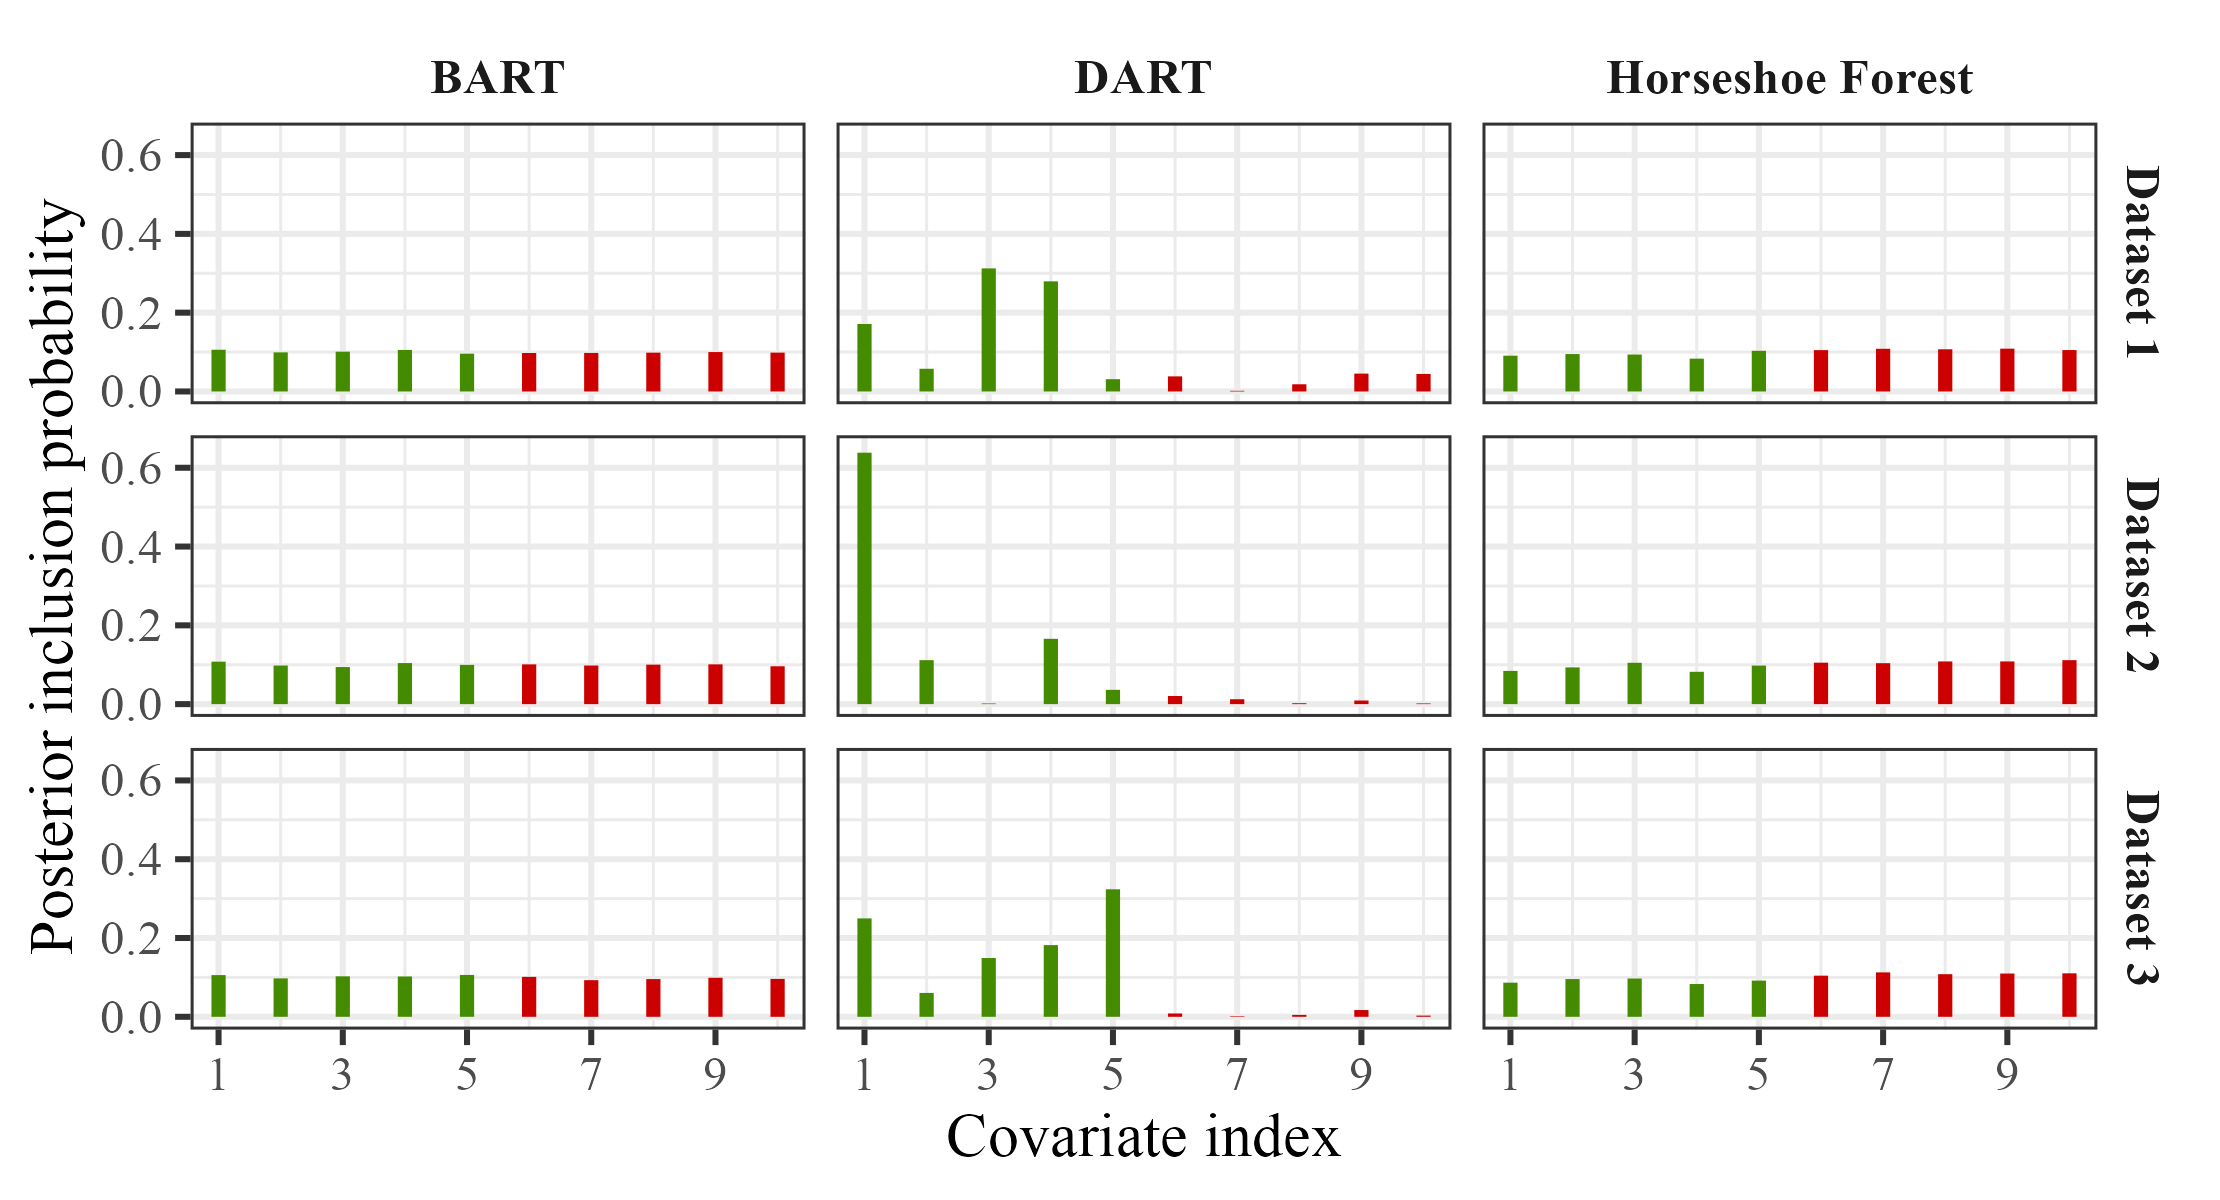
\includegraphics[width=0.85\linewidth]{revision_posterior_inclusion_plot.png}
\end{figure}

\vspace{-0.3em}
\begin{itemize}
  \item \textbf{BART} and \textbf{Horseshoe Forest}: near-uniform splitting mass across covariates --- no structural concentration, but the Horseshoe Forest shrinks uninformative step height contributions to near zero.
  \item \textbf{DART}: sharp Dirichlet-driven concentration, but across replicates it can concentrate on the \emph{wrong} subset --- excluding true signal (green) in favour of noise (red).
  \item \textbf{Take-away.} Regularising \emph{which} covariates split is brittle; regularising the \emph{magnitude} of each local effect step heights structural flexibility intact.
\end{itemize}
\end{frame}

\begin{frame}{}
\end{frame}

\end{document}